\documentclass[border={5pt 0pt}]{standalone}

\usepackage{xcolor}
\definecolor{fgcolor}{HTML}{f0f6fc}
\definecolor{bgcolor}{HTML}{0d1117}
\definecolor{myblue}{HTML}{1d597f}
\definecolor{myorange}{HTML}{b27b43}
\definecolor{mygreen}{HTML}{699963}
\colorlet{mygray}{gray!50!black}

\usepackage{tikz}
\usepackage{tikz-timing}
\usetikzlibrary{fit, positioning, shapes.geometric, shapes.symbols, backgrounds}

\newlength{\vhdlregh}\setlength{\vhdlregh}{2em}
\newlength{\vhdlregw}\setlength{\vhdlregw}{1em}

\tikzset{
    text=fgcolor,
    arrow/.style={ ->, draw=fgcolor, very thick },
    % Register
    regbox/.style={ rectangle, very thick, draw=fgcolor, fill=mygray, minimum width=\vhdlregw, minimum height=\vhdlregh },
    regwedge/.style={ isosceles triangle, isosceles triangle apex angle=80, draw=fgcolor, very thick, anchor=right corner, scale=0.33 },
    register/.pic={
        \node[regbox] () {#1};
        \node[above right=0.1em and 0.05em of .south west, regwedge] (-wedge) {};
    },
    % Adder, multiplier, etc.
    adder/.style={ circle, draw=fgcolor, very thick },
    % Cloud (for combinational logic)
    mycloud/.style={ cloud, draw=fgcolor, very thick, inner sep=2pt, minimum width=0.8cm, minimum height=0.8cm },
}


\usepackage{pifont}
\newcommand{\mycheckmark}{\ding{52}}
\newcommand{\mycrossmark}{\ding{56}}

\usepackage{bm}

\begin{document}

\pagecolor{bgcolor}

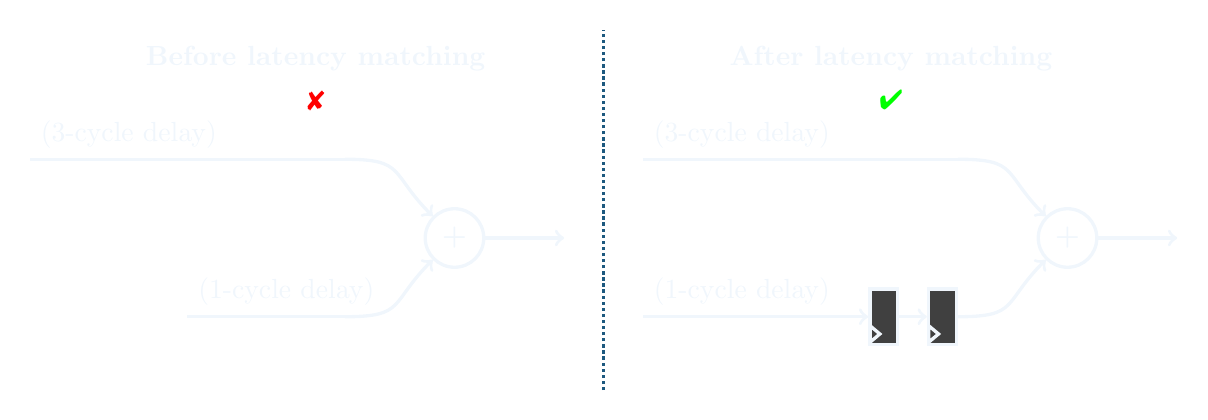
\begin{tikzpicture}
    % Before latency matching
    \coordinate (before-start);
    \coordinate[above=of before-start] (before-start-above);
    \coordinate[below=of before-start] (before-start-below);
    \coordinate[right=2 of before-start-below] (before-start-below);
    \coordinate[right=2 of before-start-below] (before-below);
    \coordinate[right=4 of before-start-above] (before-above);
    \draw[transparent] (before-above.east) to coordinate[midway] (midway) (before-below.east);
    \node[adder, right=of midway] (before-zip) {$\boldsymbol{+}$};
    \coordinate[right=of before-zip] (before-end);

    \draw[arrow, -] (before-start-above) to node[at start, above, anchor=south west] {(3-cycle delay)} (before-above);
    \draw[arrow, -] (before-start-below) to node[at start, above, anchor=south west] {(1-cycle delay)} (before-below);
    \draw[arrow, out=0, in=135, looseness=1.5] (before-above) to (before-zip);
    \draw[arrow, out=0, in=225, looseness=1.5] (before-below.east) to (before-zip);
    \draw[arrow] (before-zip) to (before-end);

    % After latency matching
    \coordinate[right=of before-end] (after-start);
    \coordinate[above=of after-start] (after-start-above);
    \coordinate[below=of after-start] (after-start-below);
    \coordinate[right=4 of after-start-above] (after-above);
    \coordinate[right=4 of after-start-below] (after-below);
    \draw[transparent] (after-above.east) to coordinate[midway] (midway) (after-below.east);
    \node[adder, right=of midway] (after-zip) {$\boldsymbol{+}$};
    \pic[left=0pt of after-below] (reg-2) {register};
    \pic[left=1em of reg-2] (reg-1) {register};
    \coordinate[right=of after-zip] (after-end);

    \draw[arrow, -] (after-start-above) to node[at start, above, anchor=south west] {(3-cycle delay)} (after-above);
    \draw[arrow] (after-start-below) to node[at start, above, anchor=south west] {(1-cycle delay)} (reg-1);
    \draw[arrow, out=0, in=135, looseness=1.5] (after-above) to (after-zip);
    \draw[arrow] (reg-1) to (reg-2);
    \draw[arrow, out=0, in=225, looseness=1.5] (reg-2) to (after-zip);
    \draw[arrow] (after-zip) to (after-end);

    % Separator
    \draw[transparent] (before-end) to coordinate[midway] (vrule-mid) (after-start);
    \coordinate[above=7em of vrule-mid] (vrule-top);
    \coordinate[below=5em of vrule-mid] (vrule-bot);
    \draw[arrow, -, myblue, densely dotted] ([xshift=0pt, yshift=-5pt] vrule-bot) to ([xshift=0pt, yshift=5pt] vrule-top);

    % "Before" title
    \draw[transparent] (current bounding box.north west) to coordinate[midway] (before-title) (vrule-top);
    \node[below=0pt of before-title] (before-title) {\textbf{Before latency matching}};
    \node[below=0pt of before-title, text=red] {\mycrossmark};

    % "After" title
    \draw[transparent] (current bounding box.north east) to coordinate[midway] (after-title) (vrule-top);
    \node[below=0pt of after-title] (after-title) {\textbf{After latency matching}};
    \node[below=0pt of after-title, text=green] {\mycheckmark};
\end{tikzpicture}

\end{document}
